\label{chapter:experiments}
 
Language model neural network artichecture is adopt from \href{https://github.com/pytorch/examples/tree/master/word_language_model}{pytorch/examples} project. Tokenizer codes and models are replaced with Part 2 and vocab for Language Modeling is construct in part 2. In this part the corpus is divided into three part, train set, dev set and test set. LanguageModel is trained on each label separately to evaluate capability of each model to generate specific news. Models are saved in "models/lm" directory. 
Models are trained on GTX1070 GPU. training process is 10 time faster than CPU. 
\section{LSTM}
Use LSTM architecture(Figure \ref{fig:mylstm}) for language model. Best perplexity recorded is 47 on "Science" label. Each epoch last about 0.36 second, perplexity method starts from 60 and it is 43 on validation data on last epoch.\ref{fig:lstm_education}

\begin{figure}
	\centering
	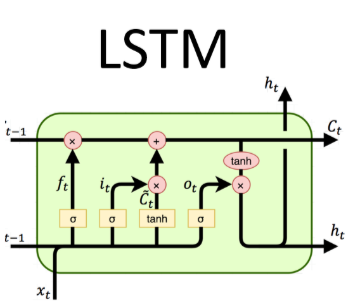
\includegraphics[width=10cm]{images/lstm.png}
	\caption{LSTM Architecture}
	\label{fig:mylstm}
	
\end{figure}

\begin{figure}
	\centering
	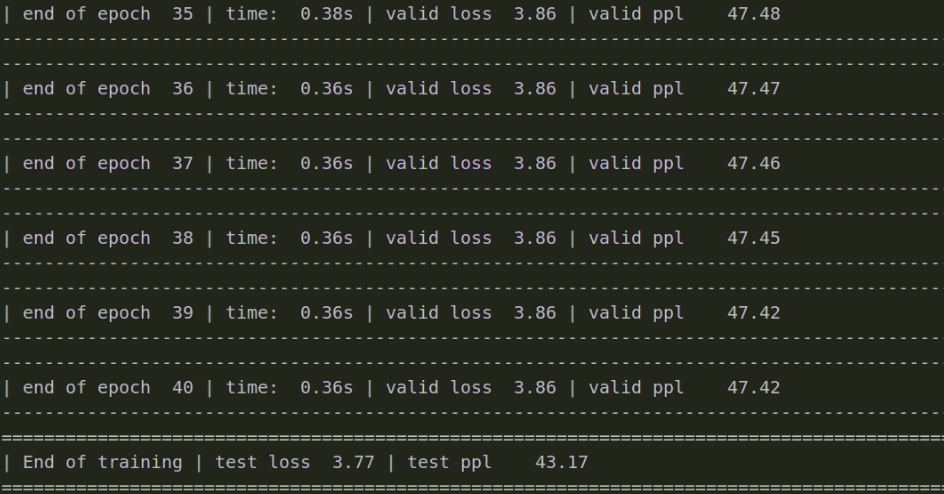
\includegraphics[width=10cm]{images/lstm_danesh.png}
	\caption{Perplexity LSTM language model, label = Science}
	\label{fig:lstm_education}
\end{figure}

In this trial, there are many <unk> token in output generated text. But generated sentences are in "Science" context.\ref{fig:gru_education_out}
\begin{figure}
	\centering
	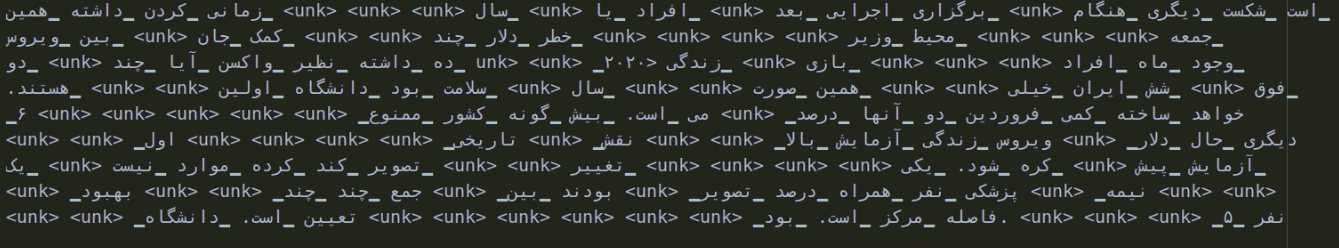
\includegraphics[width=15cm]{images/lstm_danesh_out.png}
	\caption{Generated Text LSTM language model, label = Science}
	\label{fig:gru_education_out}
\end{figure}

\section{GRU}

Use GRU architecture (Figure \ref{fig:mygru}) for language model. Few Last epochs and output is illustrated in figure \ref{fig:gru_education}. LSTM and GRU have similar learning power as a evidence perplexity of GRU model on test set is 43, when label is "Science", same as LSTM. Each epoch last about 0.33 second as expected GRU model is faster, compare to LSTM model. 


\begin{figure}
	\centering
	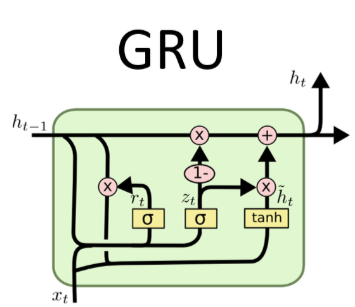
\includegraphics[width=10cm]{images/gru.png}
	\caption{GRU Architecture}
	\label{fig:mygru}
	
\end{figure}

\begin{figure}
	\centering
	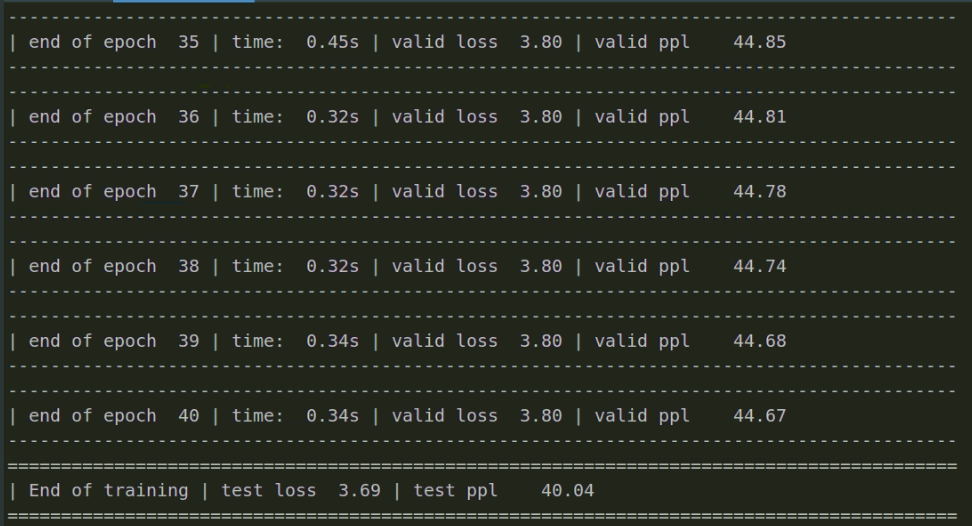
\includegraphics[width=10cm]{images/gru_danesh.png}
	\caption{Perplexity GRU language model, label = Science}
	\label{fig:gru_education}
\end{figure}

In this trial, again there are many <unk> token in output generated text. Generated sentences are in "Education" context.\ref{fig:gru_edu_out}

\begin{figure}
	\centering
	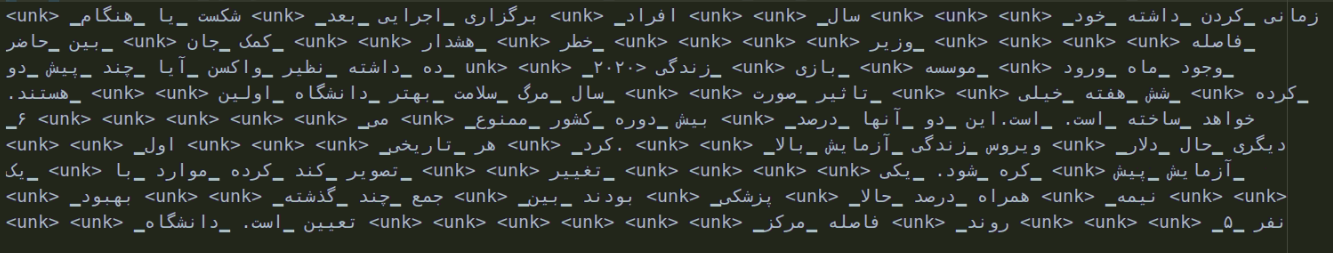
\includegraphics[width=15cm]{images/gru_danesh_out.png}
	\caption{Generated Text GRU language model, label = Science}
	\label{fig:gru_edu_out}
\end{figure}

\section{Transformer}
In last trial Transformer architecture is used for language model. This model construct of a \b{Encoder} and \b{Decoder}. Encoder consist Embedding layer and Decoder consists Linear layer. Few Last epochs and output is illustrated in figure \ref{fig:transformer_edu}. LSTM and GRU both have almost similar learning power, but with transformer architecture it is possible to access better results. As shown in Figure \ref{fig:transformer_edu_out} test perplexity is 37.41, when label is "Science" which is 3 score better than previous models. Each epoch last longer than previous models and it is about 0.40 second.
 
\begin{figure}
	\centering
	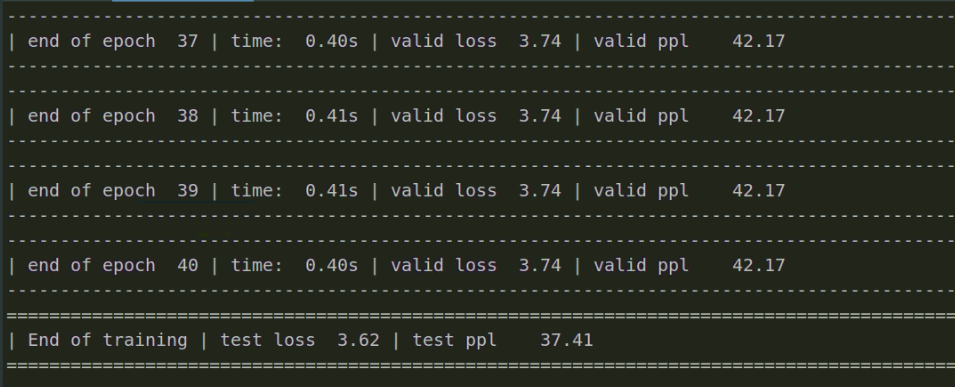
\includegraphics[width=10cm]{images/transformer_danesh.png}
	\caption{Perplexity Transformer language model, label = Science}
	\label{fig:transformer_edu}
\end{figure}

In this trial generated text is shown in \ref{fig:transformer_edu_out}. Number of <unk> token is decreased and there are more meaningful sentences. Generated sentences are in "Science" context.
\begin{figure}
	\centering
	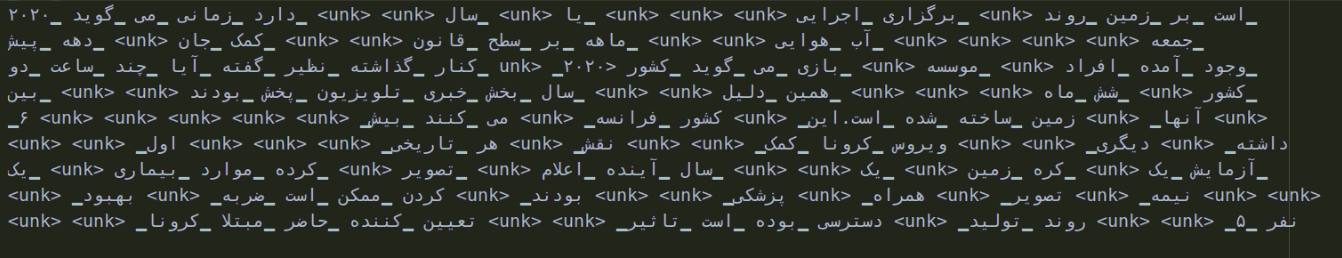
\includegraphics[width=15cm]{images/transformer_danesh_out.png}
	\caption{Generated Text Transformer language model, label = Science}
	\label{fig:transformer_edu_out}
\end{figure}

Run "bash run.sh 4" to train all three types of language models. Models will save in "models/lm" directory. Then run "bash run.sh 41" in order to generate text for each label. For each model generated text will save in corresponding file in "reports/lm" directory.

\section{Temperature}
Different temperature can be used when generating text. If set temperature low, generated text will be more general, as a result number of <unk> token will increase. On the other hand by setting higher value for temperature model diversity increases. For this project 1 is best choice for temperature parameter.
    
\section{Final Outputs} 
In this section output of each label on trained transformer-based language model is represented. 
\subsection{Iran}
Iran news is largest corpus in this dataset. We can see more meaningful sentences and less <unk> tokens. Generated sentences seems link Iran news and generated-words illustrated in Figure \ref{fig:iran} are related to the context. 
\begin{figure}
	\centering
	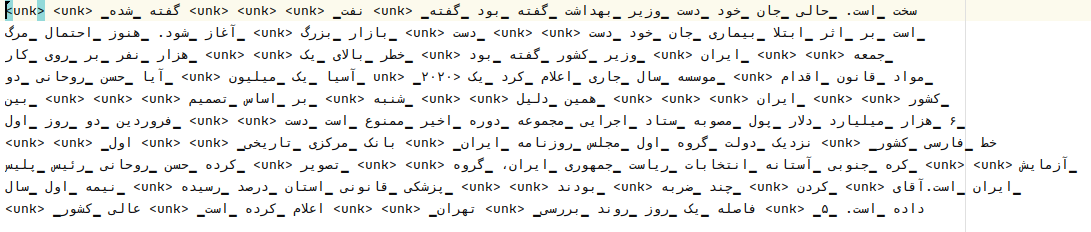
\includegraphics[width=15cm]{images/iran.png}
	\caption{Generated Text Transformer language model, label = Iran}
	\label{fig:iran}
\end{figure}

\subsection{Art}
Longest n-gram in generated text without any <unk> token is placed on second line, which n is equal to 10(Figure \ref{fig:art}). This sequence of words is not meaningful enough, but seems fluent. 
\begin{figure}
	\centering
	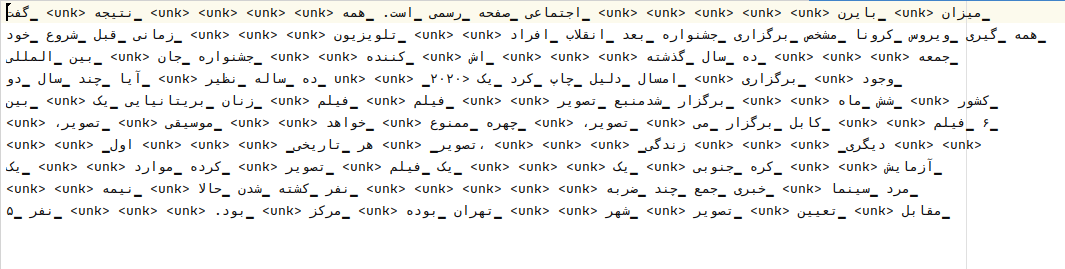
\includegraphics[width=15cm]{images/art.png}
	\caption{Generated Text Transformer language model, label = Art}
	\label{fig:art}
\end{figure}
\subsection{Science}
In this section there are many <unk> tokens due lack of data in Science class. Longest sequence of words is 4-grams and used words are more general than other sections.
\begin{figure}
	\centering
	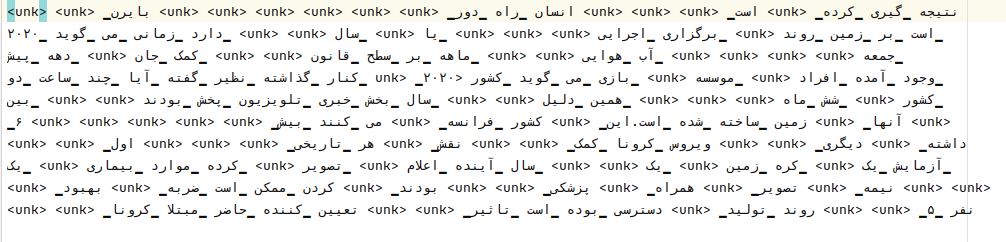
\includegraphics[width=15cm]{images/science.png}
	\caption{Generated Text Transformer language model, label = Science}
	\label{fig:science}
\end{figure}
\subsection{Economic}
In Economic class generated field as it is shown in figure \ref{fig:economic} most at least 6-grams are construct of meaningful sequences of words and they sounds same as economic news. We can see many 8-grams without any <unk> token in this section. 
\begin{figure}
	\centering
	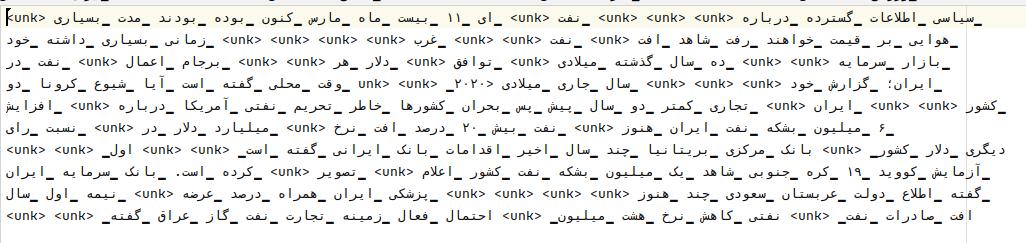
\includegraphics[width=15cm]{images/economic.png}
	\caption{Generated Text Transformer language model, label = Economic}
	\label{fig:economic}
\end{figure}
\subsection{Sport}
In this class, generated text includes of variety of meaningful n-grams without any <unk> token. It is interesting that fluent and meaning 9-garms sequence of words is constructed.(Line 4, Figure \ref{fig:sport})
\begin{figure}
	\centering
	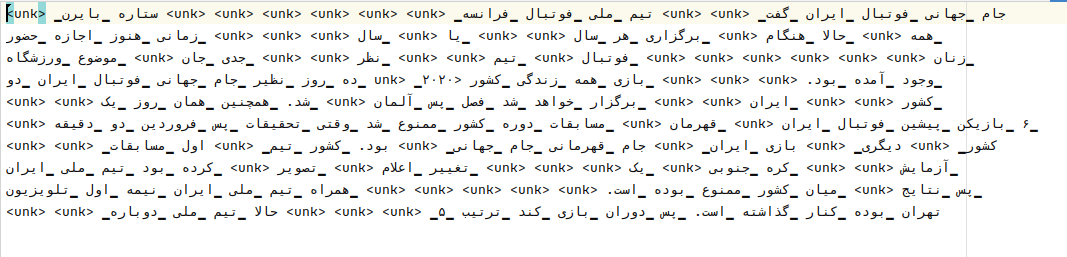
\includegraphics[width=15cm]{images/sport.png}
	\caption{Generated Text Transformer language model, label = Sport}
	\label{fig:sport}
\end{figure}
